\section{Results and Comparison}

In this chapter we are describing how we have tested and bench marked our implementations. We have tested the algorithms on two systems. The first system is the provided test system with a Tesla K10, and the second system is a personal computer with an NVIDIA RTX 2070 GPU. We are discussing the differences between the chosen strategies as well as differences regarding the GPU's.

We evaluate the implemented approaches by providing benchmarks with different sample and window sizes. 

\subsection{NVIDIA RTX 2070}

The overview in Figure~\ref{fig:group_picture_rtx2070} shows the output of the NVVP executed on the RTX 2070 test system. The green bars are marking the full computation time for each algorithm. This includes the allocation of host memory (unmarked). The allocation and transfer of/to device memory (blue), the kernel execution (yellow) and transferring the results from device to host memory (pink). Without going into the detailed numbers, we can see that the time taken for memory allocations and transfer dominates the timescale. Typically the kernel execution only takes a quarter of the overall processing time (except for the thrust implementation). 

\begin{sidewaysfigure}
    \centering
    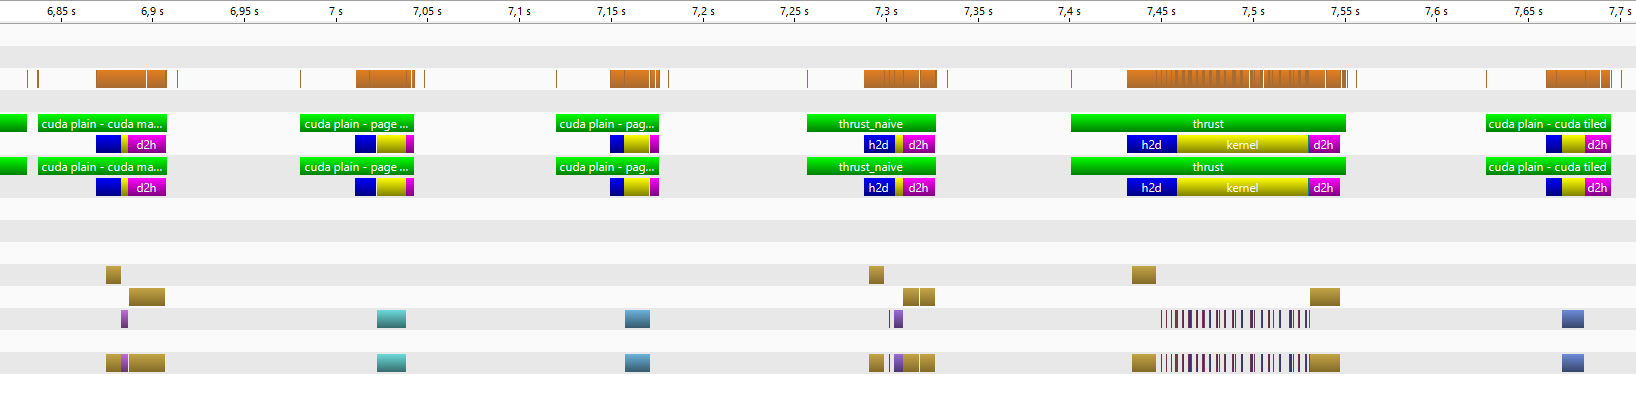
\includegraphics[width=1.0\linewidth]{Figures/group_picture_rtx2070}
    \caption{Overview of algorithms for a profiling run with a sample size of 10.000.000 and a sliding window size of 256 on the NVIDIA RTX 2070. NVTX ranges are marking the phases of each algorithm. Preparation time in blue. Kernel execution in yellow. Copying results to host in pink. Shown from left to right are: CUDA Malloc, CUDA Pagelocked, CUDA Pagelocked Shared, Thrust Naive, Thrust and CUDA Tiled}
    \label{fig:group_picture_rtx2070}
\end{sidewaysfigure}

What we can also see in this overview is that multiple kernel calls are computation wise extremely expensive, but sometimes needed to achieve a grid wide synchronization as required in the Thrust implementation (Figure~\ref{fig:group_picture_rtx2070} \#5). Multiple kernels should be avoided at all cost, and be replaced by tiling schemes which limit the requirements for synchronization to sub groups of blocks or even warps as used in the CUDA Tiling approach (Figure~\ref{fig:group_picture_rtx2070} \#6). 

\begin{figure}
    \centering
    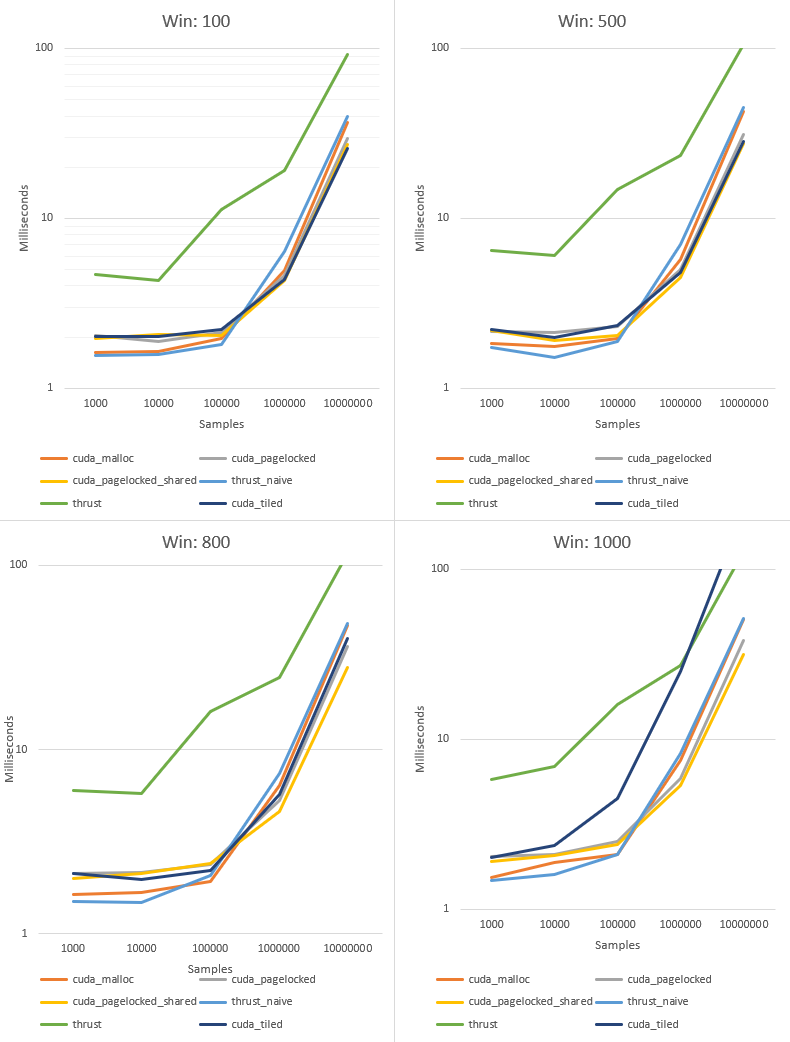
\includegraphics[width=1.0\linewidth]{Figures/rtx2070_ms_vs_samples.png}
    \caption{Results for all six implementations at different window and sample sizes. We omitted Lemire as it is much slower than competitors. Duration is shown on a logarithmic scale. The \texttt{cuda\_tiled} approach appears to be very efficient for large sample sizes and small window sizes, the naive linear scan used by \texttt{cuda\_pagelocked\_shared} dominates at large window sizes.}
    \label{fig:rtx2070_ms_vs_samples}
\end{figure}

Figure~\ref{fig:rtx2070_ms_vs_samples} shows the benchmark results for the NVIDIA RTX 2070 GPU with window sizes of 100, 500, 800 and 1000 elements. We left out Lemire's approach for a better scaling of the graph. The clearly worst performing algorithm of ours was the Thrust implementation. Since global synchronization via multiple sequential kernel starts was required, the performance of this approach took a big hit. The other five approaches are performing very similarly. For smaller window sizes (100, 500) the CUDA Tiled approach performs fastest by a small margin. For larger windows (800, 1000) the naive iteration scheme performs better, and among these CUDA page-locked shared is always the fastest one.



\subsection{NVIDIA Tesla K10.G2}

The overview in Figure~\ref{fig:group_picture_tesla_k10g2} shows the output of the NVVP executed on the Tesla K10.G2 test system. Similar to the overview for the RTX 2070 test system the green bars are marking the full computation time for each algorithm. Again this includes the allocation of host memory (unmarked). The allocation and transfer of/to device memory (blue), the kernel execution (yellow) and transferring the results from device to host memory (pink).

\begin{sidewaysfigure}
    \centering
    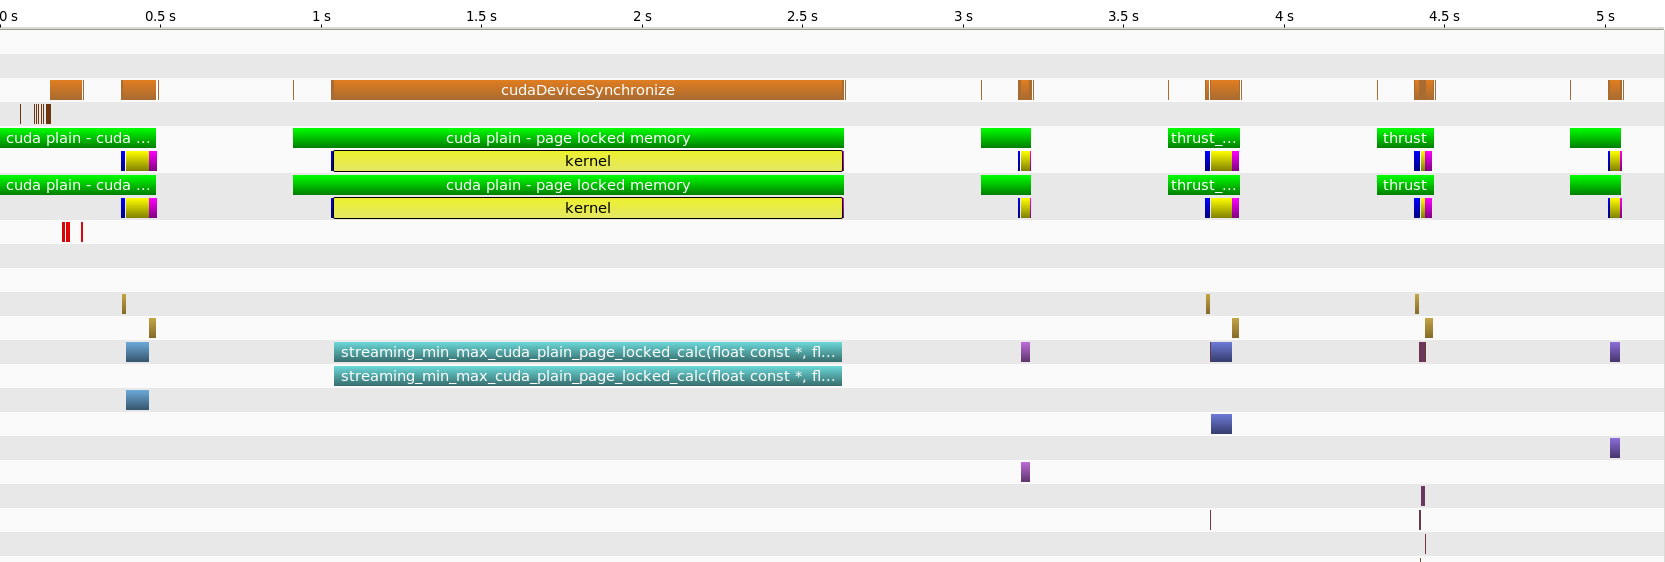
\includegraphics[width=1.0\linewidth]{Figures/group_picture_tesla_k10g2}
    \caption{Overview of algorithms for a profiling run with a sample size of 10.000.000 and a sliding window size of 256 on the NVIDIA Tesla K10.G2. NVTX ranges are marking the phases of each algorithm. Preparation time in blue. Kernel execution in yellow. Copying results to host in pink. Shown from left to right are: CUDA Malloc, CUDA Pagelocked, CUDA Pagelocked Shared, Thrust Naive, Thrust and CUDA Tiled}
    \label{fig:group_picture_tesla_k10g2}
\end{sidewaysfigure}

An obvious overall difference is that all measured times on the 
Tesla K10.G2 test system are substantially (factor 2-3) longer than those measured on the RTX 2070 test system, which is not surprising considering the specifications of both. Thus we'll now focus on relative differences between the two systems.

Interestingly in contrast to the results from RTX 2070 test system the time required for memory allocation and memory transfer is in general not at all that dominating. However, the direct access to page-locked memory on the host CPU (which manifests itself in the kernel execution time of the CUDA Pagelocked implementation) dominates the timing by at least an order of magnitude. A wild guess (which is not confirmed) is that the Tesla K10.G2 test system is inferior when it comes to combining multiple memory accesses into a single bulk transfer.
Another interesting difference in comparison to the results from the RTX 2070 test system is that the thrust implementation is en-par with the both plain CUDA implementations using shared memory for caching (which suggests that on the Tesla K10.G2 test system the Thrust library does something similar under the hood). A final interesting difference is that the tiled Thrust implementation (Thrust) outperforms the naive Thrust implementation (Thrust Naive) on the Tesla K10.G2 test system whereas on the RTX 2070 test system it's exactly the other way round.

\begin{figure}
    \centering
    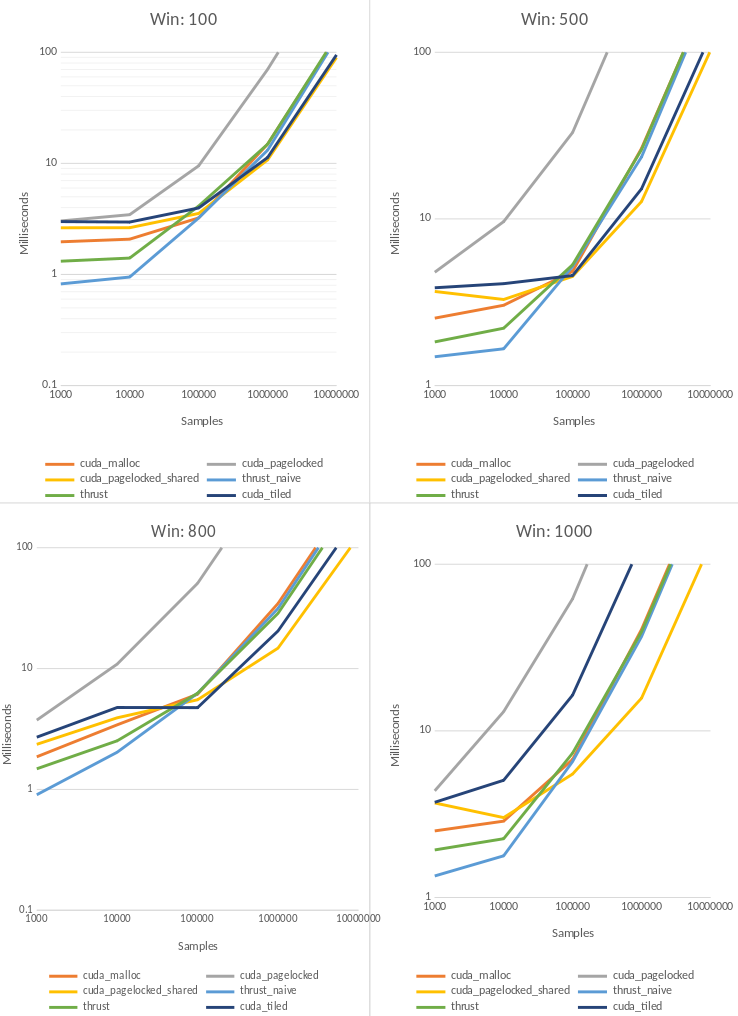
\includegraphics[width=1.0\linewidth]{Figures/tesla_k10g2_ms_vs_samples.png}
    \caption{Results for all six implementations at different window and sample sizes. Again we omitted Lemire as it is considerably slower than competitors especially with large sample sets. Duration is shown on a logarithmic scale. The \texttt{cuda\_pagelocked} approach (using the naive linear scan) is non-performing for all sample and small window sizes. The \texttt{cuda\_pagelocked\_shared} (which uses the naive linear scan as well) dominates at large window sizes.}
    \label{fig:tesla_k10g2_ms_vs_samples}
\end{figure}

Figure~\ref{fig:tesla_k10g2_ms_vs_samples} shows the benchmark results for the NVIDIA Tesla K10.G2 GPU with window sizes of 100, 500, 800 and 1000 elements. Again we left out Lemire's approach for a better scaling of the graph. The clearly worst performing algorithm on this test system was the CUDA page-locked implementation (without using shared memory as a cache) for all sample and sliding windows sizes. The hypothesized cause of this is the lack of capability to combine multiple memory accesses into a single bulk transfer. The CUDA tiled implementation showed the second worst performance for small sample sizes, but gains on larger samples sizes as long as the window size is below a threshold of approx.\ 900. With larger sample sized the CUDA page-locked shared implementation clearly shows the best performance.

\section{Summary \& Conclusion}

In the course of this lab, we implemented several different flavors of a parallel version of sliding window minimum/maximum filter with configurable window size using NVIDIA’s parallel computing platform and programming  model  for general computing on graphical processing units (GPUs) named  CUDA. These various implementation exploited different strategies w.r.t.\ performance optimizations. We conducted comprehensive measurements with different sample sizes and various sizes of the sliding window on two different hardware platforms.

The comparison of the measurement results were not fully conclusive across these two hardware platforms meaning that optimization strategies that are beneficial for one hardware platform were counter productive for the other. One common outcome on both hardware platforms however was that a rather naive parallelized linear scan together with the use of page-locked host memory combined with shared GPU memory as a program controlled cache performed superior for larger sample sizes on both hardware platforms.

The substantial differences in the measurement results on the two hardware platforms w.r.t.\ the merit of certain optimization strategies clearly suggest that a pursuing a hybrid approach, i.e., providing various different kernels within a single executable and selecting the appropriate one during run-time based on the concrete workload and the concrete hardware platform, is a feasible approach when striving for optimal performance on a broad range of different hardware platforms and when dealing with various different workloads.